\section{NP-problemer} \label{kap:np}
Problemer kan alt efter deres tidskompleksitet inddeles i forskellige kategorier. Hvis et problem kan løses i polynomisk tid af en \emph{deterministisk} algoritme, kaldes problemet \emph{P}, som står for polynomial time.
At en algoritme er deterministisk, betyder, at man kender alle trin i algorimen, og at den ikke indeholder nogle tilfældige hændelser. En \emph{ikke-deterministisk}algoritme indeholder, i modsætning til den deterministiske, tilfældige hændelser, som kan have kendte sandsynligheder. Her kender vi ikke alle trin, algoritmen skal gennemføre. Et problem løst med denne type algoritme, i polynomisk tid, kaldes \emph{NP}, hvilket står for Non-deterministic Polynomial time. Et problem kaldes NP, hvis vi endnu ikke har fundet en effektiv, deterministisk algoritme, der kan løse disse problemer. 

P-problemer hører dog også under NP-problemer, som den delmængde af problemer, der netop godt kan løses deterministisk. 
Der er stor debat om hvorvidt, alle problemer i NP kan løses med en deterministisk algoritme, og problemer, vi troede var NP for nogle år siden, har nu en sådan algoritme. Det er dog stadig uklart, om alle NP-problemer kan løses med deterministiske algoritmer.
Vi så i \autoref{kap:kompleksitet} nogle eksempler på algoritmer med polynomisk kompleksitet. Vi ved fx, at den lineære søgning, den binære søgning, bubblesortering og indskudssortering er deterministiske algoritmer, som løser problemer i polynomisk tid og dermed løser P-problemer.

%------------------------------------------ rettet opad herfra.
Probelmer kan yderligere inddeles i underkategorier. Et problem kan nemlig også være \emph{NP-hard} og \emph{NP-complete}. Et problem kaldes NP-hard, hvis problemet kan løses af en algoritme, som kan oversættes til en løsning af alle andre NP-problemer. Det er altså meget vanskelligt at vise om et problem er NP-hard. Hvis et problem er NP-hard, kan det kun løses i polynomisk tid ved brug af ikke-determinisme, hvilket betyder at et problem ikke både kan være NP-hard og P.
Hvis et problem både er NP og NP-hard, kaldes det et NP-complete-problem. Hvis et NP-complete-problem kan løses i polynomisk tid, betyder det, at alle problemer i NP kan løses i polynomisk tid. Hvis vi eksempelvis har et NP-complete-problem, A, og B kan reduceres til A i polynomisk tid, så vil A også være et NP-complete-problem. Der findes mange NP-complete-problemer, men det er endnu ikke lykkedes at løse nogen af dem effektivt. De forskellige problemtyper ses illustreret herunder:

\begin{figure}[H]
\centering
	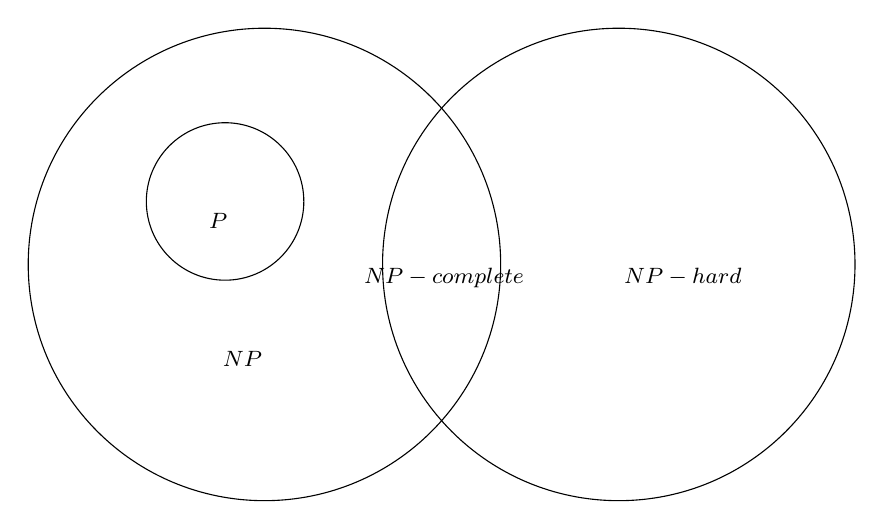
\begin{tikzpicture}
      \draw (0,2) circle (3cm);
      \put(-15,20){{\footnotesize $NP$}};
      \draw (4.5,2) circle (3cm);
      \put(130,50){{\footnotesize $NP-hard$}};
      \draw (-0.5,2.8) circle (1cm);
      \put(-20,70){{\footnotesize $P$}};
      \put(36,50){{\footnotesize $NP-complete$}};
	\end{tikzpicture}
	\caption{P, NP, NP-hard og NP-complete.}
	\label{fig.dijkstraexmp}
\end{figure}

Hvis vi kigger på Dijkstras algoritme i \autoref{kap:dijkstras}, ser vi, at denne algoritme løser problmer af typen P. Problemerne løses deterministisk og i polynomisk tid. Dette skyldes at korteste vej-problemer har optimale substrukturegenskaber. Det vil sige, at hvis en knude, $x$ er i den korteste vej fra startknuden, $u$, til endeknuden, $v$, så vil den korteste vej fra $u$ til $v$ bestå af den korteste vej fra $u$ til $x$ og den korteste vej fra $x$ til $v$. 

Dijkstras algoritme løser korteste vej-problemer, men hvad hvis vi ønsker, at finde den længste ikke-cykliske vej igennem en graf? Dette er et NP-hard-problem. Her er der nemlig ikke optimal substruktur. Vi tager et eksempel:

\begin{exmp} \label{exmp.np}
\begin{figure}[H]
\centering
	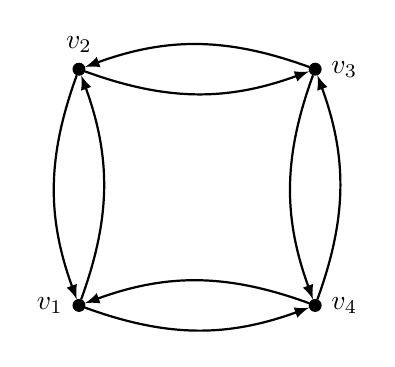
\begin{tikzpicture}

      \tikzset{enclosed/.style={draw, circle, inner sep=0pt, minimum size=.15cm, fill=black}}
%% Vertices
      	\node[enclosed, label={left: $v_1$}] (v1) at (0,0) {};
      	\node[enclosed, label={above: $v_2$}] (v2) at (0,3) {};
    		\node[enclosed, label={right: $v_3$}] (v3) at (3,3) {};
  	    \node[enclosed, label={right: $v_4$}] (v4) at (3,0) {};
%Edges
		\path [->, >=latex, thick](v1) edge [bend right=20] (v2);
		\path [->, >=latex, thick](v2) edge [bend right=20] (v1);
		\path [->, >=latex, thick](v2) edge [bend right=20] (v3);
		\path [->, >=latex, thick](v3) edge [bend right=20] (v2);
		\path [->, >=latex, thick](v3) edge [bend right=20] (v4);
		\path [->, >=latex, thick](v4) edge [bend right=20] (v3);
		\path [->, >=latex, thick](v1) edge [bend right=20] (v4);
		\path [->, >=latex, thick](v4) edge [bend right=20] (v1);

	\end{tikzpicture}
	\caption{Graf til illustration af korteste- og længste vej-problem.}
	\label{fig.multi}
\end{figure}

Vi ønsker at finde den længste vej fra $v_1$ til $v_3$. Der er to lige lange veje, nemlig $P_{1,2,3}=(v_{1},v_{2},v_{3})$ og $P_{1,4,3}=(v_{1},v_{4},v_{3})$. Hvis der havde været optimal substruktur, havde den længste vej, $P_{1,2,3}$ bestået af den længste vej fra $v_{1}$ til $v_{2}$ og den længste vej fra $v_{2}$ til $v_{3}$, men dette er ikke tilfældet. Den længste vej igennem grafen fra $v_{1}$ til $v_{2}$ er nemlig $P_{1,4,3,2}=(v_{1},v_{4},v_{3},v_{2})$, og den længste vej igennem grafen fra $v_{2}$ til $v_{3}$ er $P_{2,1,4,3}=(v_{2},v_{1},v_{4},v_{3})$. 
Den korteste vej har optimal substruktur, hvilket ses ved, at den korteste vej fra $v_{1}$ til $v_{3}$ igennem $v_{2}$ er $P_{1,2,3}=(v_{1},v_{2},v_{3})$ og denne vej består af den korteste vej fra $v_{1}$ til $v_{2}$ og den korteste vej fra $v_{2}$ til $v_{3}$, nemlig $P_{1,2}=(v_{1},v_{2})$, og $P_{2,3}=(v_{2},v_{3})$. 
\end{exmp}





